\documentclass[11pt,letterpaper,twocolumn]{article}
\usepackage[utf8]{inputenc}
\usepackage[spanish]{babel}
\usepackage{amsmath}
\usepackage{amsfonts}
\usepackage{amssymb}
\usepackage{float}
\usepackage{graphicx}
\usepackage{subfigure}
\usepackage{listings}
\usepackage{verbatim}
\usepackage[left=2cm,right=2cm,top=2cm,bottom=2cm]{geometry}
\begin{document}
\title{\huge{\textbf{ Comprobación de la dependencia de la cintura de un haz gaussiano a la distancia de propagación, y calculo de los patrones de difracción de una rendija en campo lejano y cercano mediante la FFT en MATLAB.}}}
\author{\small \textit{M. Sabogal $^{1}$}\\
	\small \textit{ $^{1}$ Programa de Física, Universidad del Atlántico, Km 7 vía a Puerto Colombia, Barranquilla, Colombia}} %Código Postal 081001
\date{} 

\twocolumn[
\begin{@twocolumnfalse}
\maketitle
\begin{center}
{\rule[0mm]{160mm}{0.2mm}}
\end{center}
\begin{abstract}
\textit{Se realizo el estudio, calculo y análisis de los patrones de difracción que se producen cuando una onda plana atraviesa una rendija de tamaño finito, tanto en campo cercano como lejano mediante la FFT en MATLAB. Comprobando los resultados predichos por la teoría de difracción de Fresnel y Fraunhofer. De igual forma, mediante la FFT se corroboro la dependencia de la cintura de un la distancia de haz gaussiano a propagación en la dirección $z$. Con discrepancias menores al $1\%$ con respecto a lo predicho por la teoría de los haces gaussianos. \\
\\
\textbf{Palabras claves: Difracción, FFT, Fresnel, gaussiano.}}
\begin{center}
\textbf{Abstract} 
\end{center}
\par 
\textit{It was carried out  the study, calculation and analysis of the drifraccion patterns that occur when a plane wave go through a slit, both near and far field using the FFT in MATLAB. verifying the results predicted by Fresnel and Fraunhofer diffraction theory. Similarly, using the FFT it was corroborated the waist dependence of a Gaussian beam to the distance propagation. With discrepancies lower than $ 1 \% $ with respect to the predicted by the theory of Gaussian beams.\\
\\
\textbf{Keywords: drifraccion, FFT, Fresnal, Gaussian.}}
\end{abstract}
\begin{center}
{\rule[0mm]{160mm}{0.2mm}}
\end{center}
\end{@twocolumnfalse}
]

\section*{\normalsize{INTRODUCCIÓN}} 
La difracción juega un papel importante en muchas aplicaciones ópticas. Esta es un factor fundamental para aplicaciones que involucren alta resolución o las largas distancias de propagación como el radar láser,
y en las aplicaciones de la participación de las pequeñas estructuras como los procesos de fotolitografía. Las ecuaciones que describen este fenómeno son muy difíciles de solucionar analíticamente, por lo que el uso de la computadora ayuda a desarrollar las soluciones de las expresiones integrales con ayuda del algoritmo de la transformada rápida de Fourier (FFT, por sus siglas en inglés). Con esta ayuda se ha llegado a desarrollar métodos eficientes para la solución de diferentes tipos de problemas en la óptica electromagnética. Uno de los problemas
más comunes en óptica se presenta cuando queremos propagar una radiación en estructuras que poseen dimensiones geométricas comparables a la longitud de onda de la radiación utilizada. Aquí es cuando ocurre el fenómeno de la difracción$^{[2],[4]}$. Se desea estudiar con énfasis la difracción que se produce cuando una onda plana atraviesa una rendija de tamaño $a$, tanto en campo lejano como en campo cercano. También se desea corroborar los resultados teóricos de la dependencia de la cintura de un haz gaussiano a la distancia de propagación en la dirección $z$, utilizando la FFT de MATLAB. 
\subsection*{Transformada de Fourier}
La transformada de Fourier, denominada así por Joseph Fourier, es una transformación matemática empleada para transformar señales entre el dominio del tiempo (o espacial) y el dominio de la frecuencia, que tiene muchas aplicaciones en la física y la ingeniería. Es reversible, siendo capaz de transformarse de cualquiera de los dominios al otro. El propio término se refiere tanto a la operación de transformación como a la función que produce. La transformada de Fourier es una aplicación que hace corresponder a una función $f(t)$ con otra función $F(\omega)$ definida de la siguiente manera:\\
$$F(\omega)= \int_{-\infty}^{\infty} f(t) \exp(i \omega t)dt$$
\par 
La transformada de Fourier es básicamente el espectro de frecuencias de una función. Un buen ejemplo de eso es lo que hace el oído humano, ya que recibe una onda auditiva y la transforma en una descomposición en distintas frecuencias (que es lo que finalmente se escucha). El oído humano va percibiendo distintas frecuencias a medida que pasa el tiempo, sin embargo, la transformada de Fourier contiene todas las frecuencias del tiempo durante el cual existió la señal; es decir, en la transformada de Fourier se obtiene un sólo espectro de frecuencias para toda la función.
\subsection*{Transformada rápida de Fourier (FFT)}
La Transformada rápida de Fourier, conocida por la abreviatura FFT (del inglés Fast Fourier Transform) es un algoritmo eficiente que permite calcular la transformada de Fourier discreta (DFT) y su inversa. La FFT es de gran importancia en una amplia variedad de aplicaciones, desde el tratamiento digital de señales y filtrado digital en general, a la resolución de ecuaciones en derivadas parciales o los algoritmos de multiplicación rápida de grandes enteros$^{[3]}$. Cuando se habla del tratamiento digital de señales, el algoritmo FFT impone algunas limitaciones en la señal y en el espectro resultante, ya que la señal muestreada y que se va a transformar debe consistir de un número de muestras igual a una potencia de dos. Sea $x(n)$ una señal aperiódica discreta en el tiempo. La transformada discreta de Fourier de esta señal se define como: 
$$X(k)= \sum_{n=0}^{N-1} x(n) \exp(i2 \pi k\dfrac{n}{N})$$
\par 
en la cual $X(k)$ es un conjunto de números complejos. Dado que la transformada discreta de Fourier inversa es análoga a la transformada discreta de Fourier, con distinto signo en el exponente y un factor 1/n, cualquier algoritmo FFT puede ser fácilmente adaptado para el cálculo de la transformada inversa discreta de Fourier$^{[3]}$. Por lo general, se define cómo:
$$x(n)= \dfrac{1}{N} \sum_{n=0}^{N-1} X(k) \exp(- i2 \pi k\dfrac{n}{N})$$
\subsection*{Ecuación paraxial de la optica}
Así como los rayos paraxiales simplificaron enormemente la óptica de rayos al permitir usar ecuaciones de propagación lineal, las ondas paraxiales son mucho más simples de tratar que las ondas en el caso general. Una onda paraxial es aquella en la que las curvas normales a los frentes de onda son rayos paraxiales. Las ondas paraxiales se propagan (más o menos) a lo largo del eje óptico, por lo que deberían estar bastante cerca de una onda plana. Por lo tanto, se puede factorizar la parte de onda plana de la onda paraxial. Para un campo eléctrico escalar que se propaga a lo largo de la dirección z$^{[1]}$:

$$E^{(+)}(r)=\psi(r)\exp(ikz) $$ 
\par 
Donde, $\psi$ es la envolvente y $\exp(ikx)$ es la parte correspondiente a la propagación. Para una onda paraxial, la envolvente $\psi$ debe ser suave en la escala de $\lambda$. Introduciendo esto en la ecuación de onda (Helmholtz), $(\nabla^{2}+k^{2})E^{(+)}=0$, se encuentra:\\
 
$$\left( \nabla^{2}_{T} + \textit{i}2k \dfrac{\partial}{\partial z}+\dfrac{\partial^{2}}{\partial z^{2}} \right)\psi=0$$ 
\par 
Donde $\nabla^{2}:=\dfrac{\partial^{2}}{\partial x^{2}}+\dfrac{\partial^{2}}{\partial y^{2}}$ es el laplaciano transversal. Si $\psi$ es suave (es decir varia lentamente) en la escala de $\lambda$, por tanto:\\
$$\dfrac{\partial \psi}{\partial z} \ll \dfrac{\psi}{\lambda} \hspace*{0.1cm} \longrightarrow \hspace*{0.1cm} \dfrac{\partial \psi}{\partial z} \ll k \psi \hspace*{0.1cm} \longrightarrow \hspace*{0.1cm} \dfrac{\partial^{2} \psi}{\partial z^{2}} \ll k \dfrac{\partial \psi}{\partial z}$$
\par 
De manera que se puede despreciar el termino $\partial^{2}/{\partial z^{2}}$ en la ecuación anterior. Esto es llamado \textbf{slowly varying envelope approximation}, y la ecuación de onda resultante es la ecuacion paraxial$^{[1]}$; en nuestro caso por simplicidad, la variacion en el eje $y$ es cero, obteniendo: 
\begin{equation}
\left( \dfrac{\partial^{2}}{\partial x^{2}} + \textit{i}2k \dfrac{\partial}{\partial z}\right)\psi=0
\end{equation}
\par 
Con el fin de solucionar la ecuación paraxial, se utiliza la transformada de fourier, suponiendo la solucion de la forma: 
\begin{equation}
\psi(z,x)= \int_{-\infty}^{\infty} \hat{\psi}(z,k_{x}) exp(ik_{x}x) dk_{x}
\end{equation}
\par 
Derivando, la solución con respecto a x y z en cada caso se obtiene:  
$$\dfrac{\partial \psi}{\partial z}=  \int_{-\infty}^{\infty} \dfrac{\partial \hat{\psi}}{\partial z} exp(ik_{x}x) dk_{x}$$
$$\dfrac{\partial^{2} \psi}{\partial x^{2}}= -k_{x} \int_{-\infty}^{\infty} \hat{\psi} exp(ik_{x}x) dk_{x}$$
\par 
Remplazando en la ecuación paraxial: 
$$\int_{-\infty}^{\infty} \left[ \textit{i} \dfrac{\partial \hat{\psi}}{\partial z} -\dfrac{k_{x}}{2k}  \hat{\psi} \right] exp(ik_{x}x) dk_{x}=0$$
\par 
Debido a que $ exp(ik_{x}x)$ nunca es cero, se obtiene: 
$$\textit{i} \dfrac{\partial \hat{\psi}}{\partial z} -\dfrac{k_{x}}{2k}  \hat{\psi}=0$$
\par 
La cual es una ecuación diferencial solucionable por medio del método de separación de variable. Separando variables e integrando se tiene: 
$$\int_{\hat{\psi}(0,k_{x})}^{\hat{\psi}(z,k_{x})} \dfrac{\partial \hat{\psi}}{\hat{\psi}} = - \int_{0}^{z} \dfrac{\textit{i}k_{x}}{2k} dz $$
\par 
Obteniendo: 
\begin{equation}
\hat{\psi}(z,k_{x})=\hat{\psi}(0,k_{x}) \exp\left(- \dfrac{\textit{i}k_{x}}{2k}z\right)
\end{equation}
\par 
Donde por definición: 
$$\hat{\psi}(0,k_{x})= \dfrac{1}{2\pi}\int_{-\infty}^{\infty} \psi(0,k_{x}) \exp\left(-\textit{i}k_{x} x \right) dx$$
\par 
Remplazando en (3):
$$\hat{\psi_{o}}= \left(\dfrac{1}{2\pi} \int_{-\infty}^{\infty} \psi_{o} \exp\left(-\textit{i}k_{x} x \right) dx \right) \exp\left(- \dfrac{\textit{i}k_{x}}{2k}z\right) $$
Y luego en (2), se obtiene la solución final de la ecuación paraxial: 
$$\psi(z,x)= \dfrac{1}{2\pi} \int_{-\infty}^{\infty}  \left(\dfrac{1}{2\pi} \int_{-\infty}^{\infty} \psi(0,k_{x}) \exp\left(-\textit{i}k_{x} x \right) dx \right) $$
\begin{equation}
\hspace*{2.6cm} \times \exp\left(\dfrac{\textit{-i}k_{x}}{2k}z\right) exp(ik_{x}x) dk_{x}
\end{equation}
\subsection*{Haces gaussianos}
En las últimas décadas, el uso de rayos láser se ha generalizado. Los láseres se utilizan tanto en la ciencia como en la tecnología, desde el análisis espectroscópico hasta la lectura de códigos de barras. Los rayos láser de distintos tipos y colores tienen algunas características en común: están compuestos por una banda estrecha de longitudes de onda, al punto que podemos llamarlos ``monocromáticos" (de una sola longitud de onda), y están colimados, es decir, La energía luminosa está restringida en la dirección transversal a la dirección de propagación para formar un haz estrecho. En un plano que es transversal a la dirección de propagación, la intensidad del haz disminuye en una forma gaussiana típica.$^{[2]}$\\

Las ondas más simples son la onda plana, que tiene la forma $\cos(kx-wt)$, y la onda esférica, que tiene la forma $\cos(kR-wt)/R$. Estos son modelos útiles. El haz gaussiano ( ecuación \ref{1}) es el modelo más simple de un haz dirigido que satisface las ecuaciones de Maxwell y por tanto la ecuación de onda, al menos en la aproximación paraxial. También resulta que las salidas de los resonadores de espejo esférico y los láseres son a menudo rayos gaussianos. El haz gaussiano es igual que el paquete de ondas gaussiano en la mecánica cuántica, siendo lo suficientemente complejo como para ser interesante, pero lo suficientemente simple para ser manejable.$^{[1]}$\\

$$E^{(+)}(r)=E_{o}^{(+)} \dfrac{\omega_{o}}{\omega (z)} \exp\left[\dfrac{-r^{2}}{\omega^{2}(z)}\right] \exp\left[ ik\dfrac{r^{2}}{2R(z)}\right]$$
\begin{equation}
\hspace*{2.5 cm}\times \exp \left[ ikz-i\tan^{-1}\left(\dfrac{z}{z_{o}}\right) \right] 
\label{1}
\end{equation}
\par 
Este es el haz Gaussiano o TEM$_{0,0}$ (por “Modo transversal electromagnético”; el subíndice proviene de la jerarquía de haces de Hermite-Gauss, donde TEM$_{0,0}$ es el modo fundamental). En esta expresión, se encuentra en coordenadas polares $(r,z)$ con $r=\sqrt{x^2 + y^2}$; $E_{o}$ es, como siempre, una constante de amplitud de campo general; $z_{o}$ es una constante llamada longitud de Rayleigh (o "rango de Rayleigh") y $\omega_{o}$ es el parámetro de la cintura del haz o el radio del haz, estos dos últimos presentan la ultima relación: 
$$z_{o}=\dfrac{\pi \omega_{o}^{2}}{\lambda}$$
\par 
Si $R$ es el radio de curvatura de los frentes de onda, y $\omega$ es la cintura del haz o spot en función de $z$, de la forma:
\begin{equation}
\omega(z)=\omega_{o} \sqrt{ 1 + \left( \dfrac{z}{z_{o}}\right) ^{2}}
\end{equation}
$$R(z)=z \left[ 1+ \left( \dfrac{z}{z_{o}} \right)^{2}\right]$$
\subsection*{Perfil de intensidad}
El primer factor en la ecuación (7) es el factor de amplitud, que describe completamente el perfil de intensidad del haz gaussiano. En este sentido, este es el factor más útil para comprender el comportamiento del haz gaussiano. La intensidad es solo el módulo cuadrado de la ecuación (5), pero los otros dos factores no contribuyen:
\begin{equation}
I(r,z)=I_{o}\left[\dfrac{\omega_{o}}{\omega (z)}\right]^{2} \exp\left( \dfrac{-2r^{2}}{\omega^{2}(z)}\right)
\end{equation}
\par 
Se ha definido $I_{o}= 2|E_{o}^{(+)}|^{2}$ como la intensidad máxima del haz gaussiano (que ocurre en el centro $r=0$). Claramente, la intensidad cae en la dirección radial como una función gaussiana, de ahí el nombre "rayo gaussiano". Además, tenga en cuenta que $\omega(z)$ es una medida del ancho del haz gaussiano y se reduce al valor mínimo $\omega_{o}$, en $z=0$. Tomando ésto en consideración, si se realiza un analisis en $z=0$, se obtiene: 
\begin{equation}
I(r)=I(r,0)=I_{o} \exp\left(\dfrac{-2r^{2}}{\omega_{o}^{2}}\right)
\label{inten}
\end{equation}
\par 
Que representa la distribución de intensidades en el spot que se puede apreciar en la figura 1, donde el radio de curvatura es cero.
\begin{figure}[h!]
\begin{center}
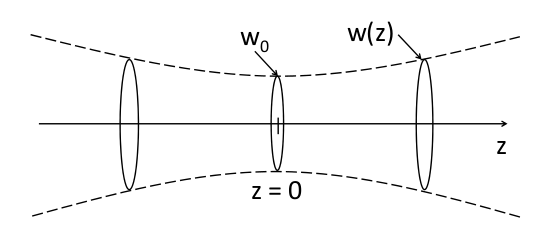
\includegraphics[scale=0.4]{spot.png}
\caption{Cintura de un haz, cuando $z=0$.$^{[5]}$}
\end{center}
\end{figure}
\par 
Finalmente, la potencia total del haz gaussiano esta dado por la integral de la intensidad sobre el plano transversal: 
\begin{equation}
P= \int_{0}^{\infty} I(r,z)2 \pi r dr= \dfrac{I_{o}}{2}\left(\pi \omega_{o}^2\right)
\end{equation}
\par 
Donde se observa que ésta es independiente tanto de $r$ como de $z$, es decir es una constante. 
\subsection*{Drifracción de Fresnel}
En física la difracción es un fenómeno característico de las ondas, éste se basa en el curvado y esparcido de las ondas cuando encuentran un obstáculo o al atravesar una rendija por ejemplo. La difracción ocurre en todo tipo de ondas, desde ondas sonoras, ondas en la superficie de un fluido, ondas electromagnéticas como la luz y las ondas de radio. La difracción de Fresnel se define como difracción de campo cercano, es un patrón de difracción de una onda electromagnética obtenida muy cerca del objeto causante de la difracción. 
\subsection*{Drifracción de Fraunhofer}
La difracción de Fraunhofer se refiere a lo que sucede con un patrón óptico después de la propagación en una distancia muy grande $z$, en la aproximación paraxial. A menudo, el ``patrón de difracción" se refiere al patrón de campo lejano de una abertura (es decir, una rendija o un orificio) iluminada por un campo monocromático uniforme, como un haz láser expandido (onda plana) en incidencia normal.${[1]}$
\subsection*{Patron de drifracción de una rendija}
Con el fin de estudiar la difracción que se produce cuando una onda plana atraviesa una rendija de tamaño $a$, tanto en campo lejano como en campo cercano, por simplicidad se analizara el caso cuando la onda es un pulso unitario de amplitud $||E_{o}^{(+)}||$, es decir un delta de Dirac. Siendo su transformada de Fouier igual a la unidad. Utilizando el teorema de la convolución y la siguiente propiedad:
$$\dfrac{1}{2\pi}\int_{-\infty}^{\infty}\left[ exp\left( \dfrac{-ik^{2}_{x}z}{2k}\right) \right]dk_{x}=\sqrt{\dfrac{k}{2 \pi i z}} \exp\left(\dfrac{ik x^{2}}{2z} \right)$$   \\
\par 
La ecuación ($4$) para el campo eléctrico, se convierte en:
$$E^{(+)}(x,z)= E^{(+)}_{o} \sqrt{\dfrac{k}{2 \pi i z}} \exp(ikz) \hspace*{4 cm} $$
$$\hspace*{3cm} \times \int_{-a/2}^{a/2} \exp\left( \dfrac{ik(x-x^{\prime})^{2}}{2z} \right) dx^{\prime}$$\\
\par 
Realizando la sustitución $x^{\prime} \longrightarrow \sqrt{\pi z/k} (x^{\prime} + x)$, se tiene: 
$$E^{(+)}(x,z)= E^{(+)}_{o} \sqrt{\dfrac{-i}{2}} \exp(ikz) \hspace*{4 cm} $$
$$\hspace*{2.5cm} \times \int_{\sqrt{\pi z/k}(-x-a/2)}^{\sqrt{\pi z/k}(-x+a/2)} \exp\left( \dfrac{i\pi x^{\prime 2}}{2z} \right) dx^{\prime}$$\\
\par 
Recordando que las integrales de fresnel son: 
\begin{equation}
C(x)=\int_{0}^{x} \cos\left(\dfrac{\pi t^{2}}{2}\right) dt \hspace*{0.3 cm} S(x)=\int_{0}^{x} \sin\left(\dfrac{\pi t^{2}}{2}\right) dt 
\end{equation}
\par 
Y utilizando el hecho de que ambas son funciones impares, porque están definidas en un intervalo de $0$ a $x$ con un integrando par, es posible reescribir el patrón de difracción de la forma: 
$$E^{(+)}(x,z)=E_{o}^{(+)} \sqrt{\dfrac{-i}{2}} \exp(ikz) \hspace*{5 cm }$$ 
\begin{equation}
\hspace*{1.6cm} \times \left[ C(A)-C(B) + iS(A)-iS(B) \right]
\end{equation}
\par 
Donde: 
\begin{equation}
A=\sqrt{\dfrac{k}{\pi z}}\left( x + \dfrac{a}{2}\right) \hspace*{0.3 cm} B=\sqrt{\dfrac{k}{\pi z}}\left( x - \dfrac{a}{2}\right)
\end{equation}
\par 
Recordando que $I=E^{(+)} E^{(+)*}$, Donde $ E^{(+)*}$ es el complejo conjugado de ($11$), se obtiene finalmente la intensidad del patrón de difracción: 
\begin{equation}
I=\dfrac{||E^{(+)}_{o}||^{2}}{2} \left( \left[C(A)-C(B)\right]^{2} + \left[ S(A)-S(B)\right]^{2} \right)
\end{equation}
\section*{-Implementación, interpretación física y resultados}
Con el fin de corroborar los resultados teóricos de la dependencia de la cintura de un haz gaussiano a la distancia de propagación en la dirección $z$, se propago un haz gaussiano, descrito por la ecuación ($5$) cuando $z=0$, mediante las herramientas computacionales de MATLAB y su FFT.\\
\par 
En primera instancia se establecieron los parámetros de la onda de estudio, cómo $\lambda$, $k$ y la cintura inicial del haz $\omega_{o}$. Posteriormente se definió el intervalo espacial de muestreo [$-x_{f},x_{f}$] mediante la función \textit{linspace()}, y el numero $N$ de particiones o numero de muestras de éste (con preferencia a ser un múltiplo de 2). Donde $x_{f}$ se definió como 5 veces la cintura ($\omega_{o}$) del haz inicial, con el propósito de tener un rango que contuviera información significativa a medida que el pulso se dispersa. A partir de esto, se definió la condición inicial como un haz gaussiano descrito por la ecuación ($5$) cuando $z=0$. Para determinar las frecuencias discretas (en nuestro caso espacial las $k_{x}$) en las cuales se va a evaluar la transformada, se definió un vector $n$ desde $-N/2$ hasta $N/2$ con el paso igual a la unidad, permitiendo encontrar las $k_{x}$ mediante la relación $k_{x}=2 \pi n/dx$, donde $dx$ es el paso del intervalo espacial de muestreo. Observado que el vector resultante $k_{x}$ presenta $N+1$ componentes, debido al tamaño y simetría del vector $n$, se removió uno de los términos de los extremos repetido.\\
\par 
Posteriormente con los parámetros y condiciones iniciales ya establecidas, se obtuvo la transformada de Fourier del haz gaussiano inicial mediante la función \textit{fft()} de MATLAB. Con la intención de apreciar y trabajar con la onda transformada, se utiliza la función \textit{fftshift()}, la cual reordena los datos obtenidos, debido a que por el funcionamiento interno del algoritmo de la función \textit{fft()}, éstos son organizados para optimizar el proceso. Al graficar el valor absoluto de la transformada reorganizada, se observa que en la figura 2 (b.), que ésta es similar a un delta de Dirac, concordando con lo establecido por la teoría.\\  
\begin{figure}[h!]
\begin{center}
\subfigure[] {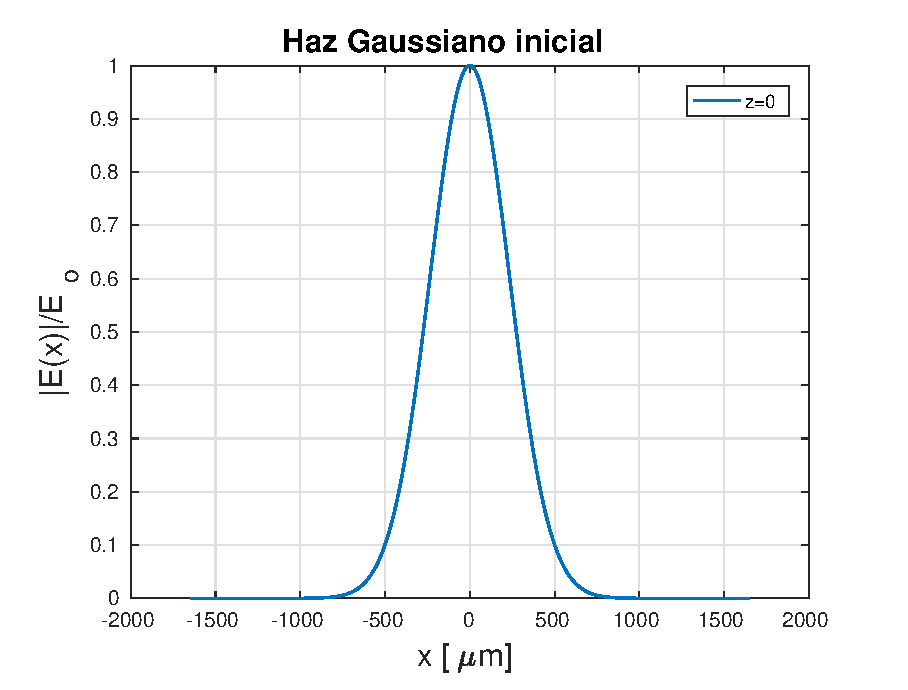
\includegraphics[scale=0.6]{H1.eps}}
\subfigure[] {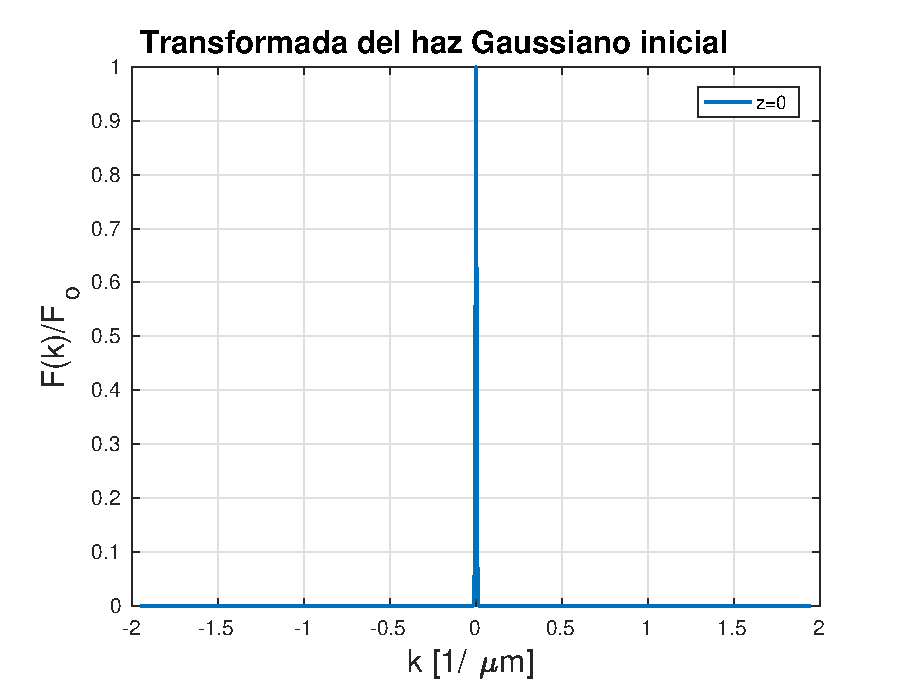
\includegraphics[scale=0.6]{T1.eps}}
\caption{(a.) Haz gaussiano con $w_{o}= 330$ $[\mu m]$; (b.) Transformada de fourier del haz.}
\end{center}
\label{pos}
\end{figure}
\par 
Siguiendo el protocolo en la ecuación (3) para solucionar la ecuación paraxial, se multiplico a la transformada inicial reorganizada por el factor propagador $\exp(-i k_{x}^{2}z/2k)$, que depende directamente de $z$ siendo esta la distancia de propagación. Posteriormente con el fin de obtener la transformada inversa de la onda propagada, se utilizo previamente la función \textit{ifftshift()} para devolver el orden dado por la función \textit{fft()}, y consecutivamente utilizar la función \textit{ifft()}, para obtener la transformada inversa, es decir el campo eléctrico de la onda propagada. Finalmente al graficar el valor absoluto del campo eléctrico al cuadrado, tanto para el haz inicial ($z=0$) cómo para el propagado una distancia $z$, se observa en la figura (3), como al propagarse la onda se dispersa, es decir aumenta la cintura del haz.\\
\begin{figure}[h!]
\begin{center}
\subfigure[] {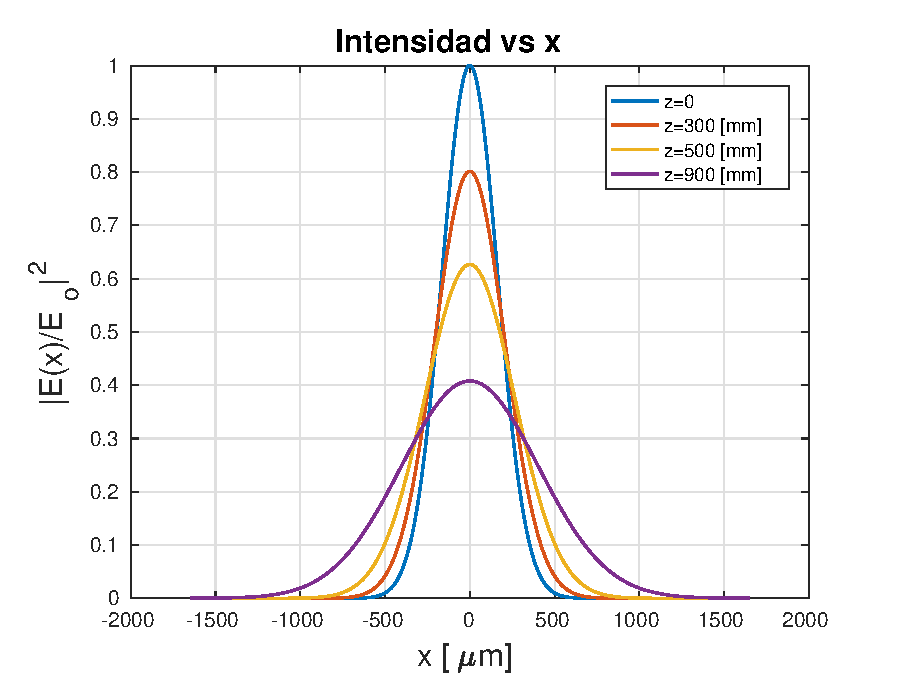
\includegraphics[scale=0.6]{propagacion.eps}}
\subfigure[] {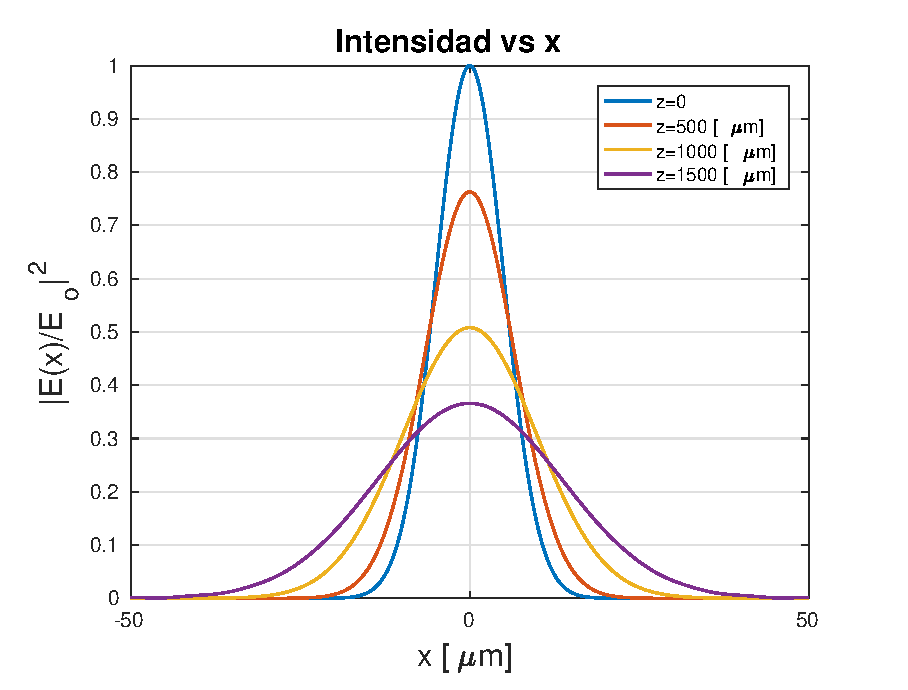
\includegraphics[scale=0.6]{propagacion2.eps}}
\caption{Graficas en las que se observa la dependencia de $\omega$ con respecto a $z$ (a.) $\omega_{o}=300$ $[\mu m]$ y (b.) $\omega_{o}=10$ $[\mu m]$}
\end{center}
\label{pos}
\end{figure}
\par 
Con la finalidad de comparar las cinturas obtenidas con los datos teóricos de la variación de la cintura del haz en función de $z$, de la ecuación (6), se realizo un \textit{fitting} modelado por la ecuación (8), a cada una de las curvas de intensidad de la figura (3), obteniendo los resultados presentes en el cuadro 1. Observando como la cintura del haz $\omega_{E}$ encontrada, presenta una diferencia menor al $1\%$ con respecto al valor teórico calculado por medio de la ecuación (6) en cada caso.\\  
\begin{table}[h!]
\begin{center}
\begin{tabular}{|c|c|c|c|}
  \hline
  \multicolumn{4}{|c|}{(a.) $\lambda=850$ $[nm]$; $\omega_{o}= 330$ $[\mu m]$ } \\ 
  \hline 
  $z$ $[mm]$ & $\omega_{E}(z)$ $[\mu m]$ & $\omega_{T}(z)$ $\mu m$ & $\%$ \\ 
  \hline 
  300 & 411.726 & 411.582 & 0.035 \\ 
  \hline 
  500 & 526.577 & 526.265 & 0.059\\ 
  \hline 
  900 & 808.989 & 808.331 & 0.082 \\ 
  \hline 
  \multicolumn{4}{|c|}{(b.) $\lambda=532$ $[nm]$; $\omega_{o}= 10$ $[\mu m]$ } \\ 
  \hline 
  $z$ $[\mu m]$ & $\omega_{E}(z)$ $[\mu m]$ & $\omega_{T}(z)$ $\mu m$ & $\%$ \\ 
  \hline 
  500 & 13.1084 &  13.103 & 0.041 \\ 
  \hline 
  1000 & 526.577 & 19.666 & 0.073\\ 
  \hline 
  1500 & 27.322 & 27.298 & 0.087 \\ 
  \hline 
 \end{tabular}  
 \caption{Comparación de los datos obtenidos}
\end{center}
\end{table}
\par
Una vez se ha verificado que a partir del algoritmo y de la metodología utilizada, es posible obtener datos con una buena aproximación, se desea calcular los patrones de difracción que se producen cuando una onda plana atraviesa una rendija de tamaño $a$, tanto en campo lejano como en el cercano. Para lograr esto, se tomó como condición inicial un haz gaussiano, que impacta con una rendija de tamaño $a$, donde $\omega_{o} \gg a$, del cual solo logra atravesar la información contenida espacialmente entre $[-a/2,a/2]$, simulando un pulso unitario o un delta de Dirac.\\
%\begin{figure}[h!]
%\begin{center}
%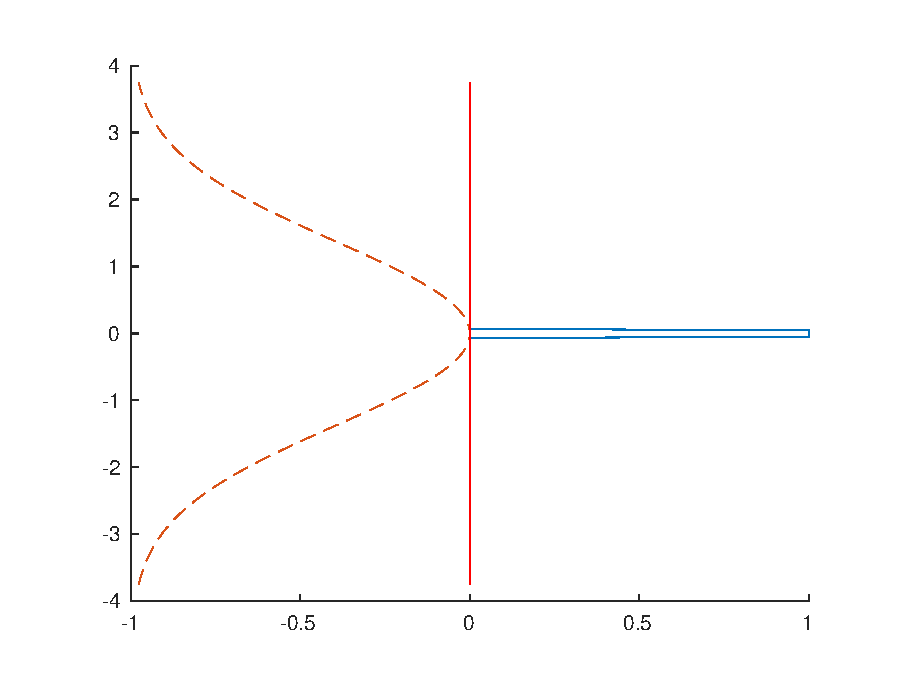
\includegraphics[scale=0.6]{Re.eps}
%\caption{}
%\end{center}
%\label{pos}
%\end{figure} 
\par 
Utilizando la metodología anterior (la utilizada para corroborar la teoría de haces gaussianos), se propago la condición inicial del pulso unitario descrita previamente, obteniendo el patrón de difracción presente en la figura (4):
\begin{figure}[h!]
\begin{center}
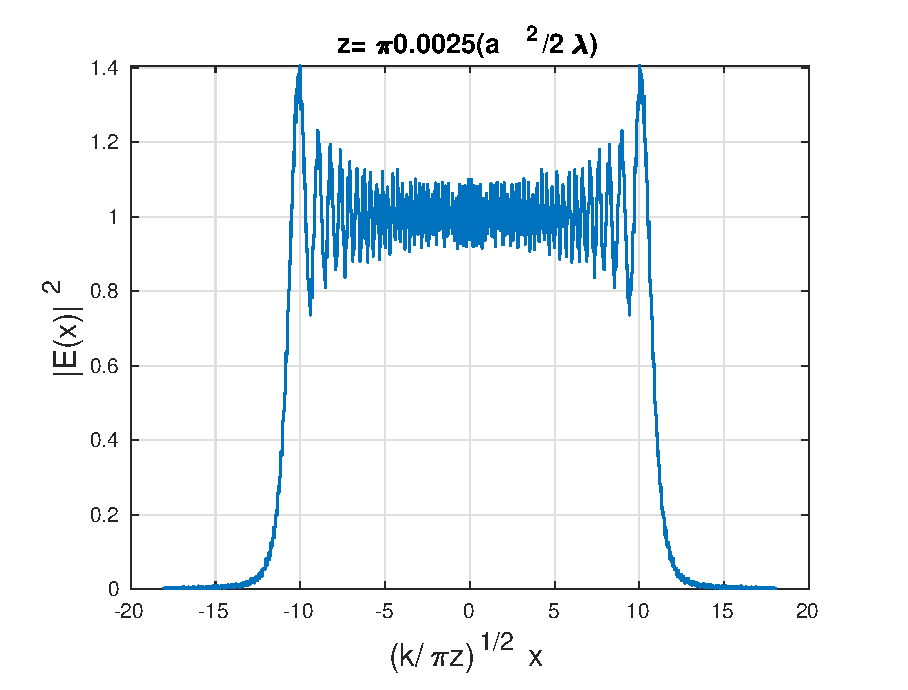
\includegraphics[scale=0.55]{p1.eps}
\caption{$a=0.075$ $[\mu m]$ y $\lambda=0.850$ $[\mu m]$}
\end{center}
\label{pos}
\end{figure} 
\par 
En harás de comprobar la veracidad de estos resultados, se resolvió el problema analítico planteado en la ecuación ($13$). Para resolver dicha ecuación, fue necesario desarrollar algoritmos que permitieran calcular las integrales de fresnel para cada punto de evaluación en $x$, obteniendo los siguientes resultados referente a éstas integrales:
\begin{figure}[h!]
\begin{center}
\subfigure[] {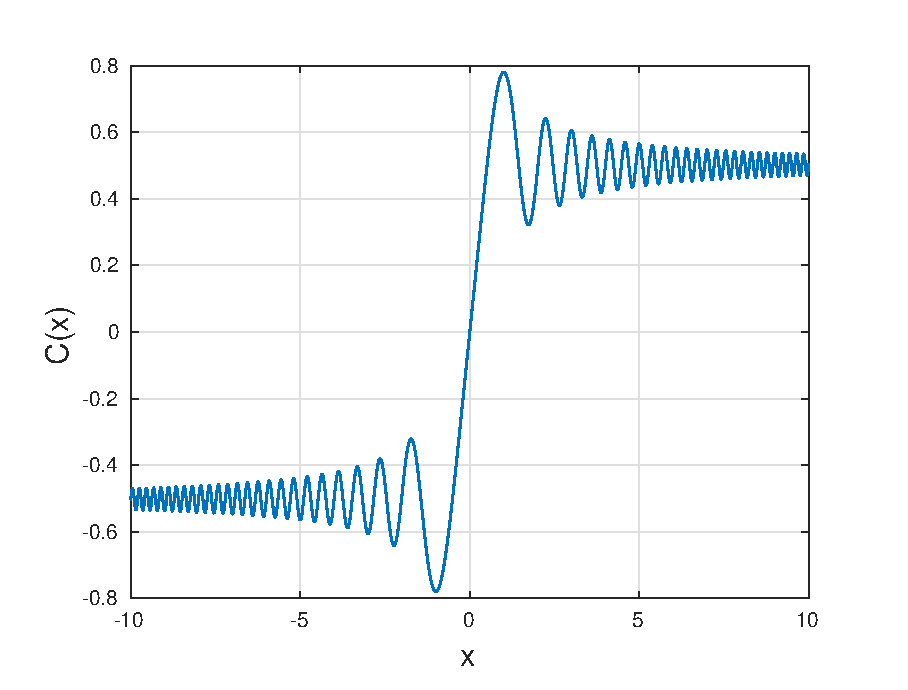
\includegraphics[scale=0.5]{fre1.eps}}
\subfigure[] {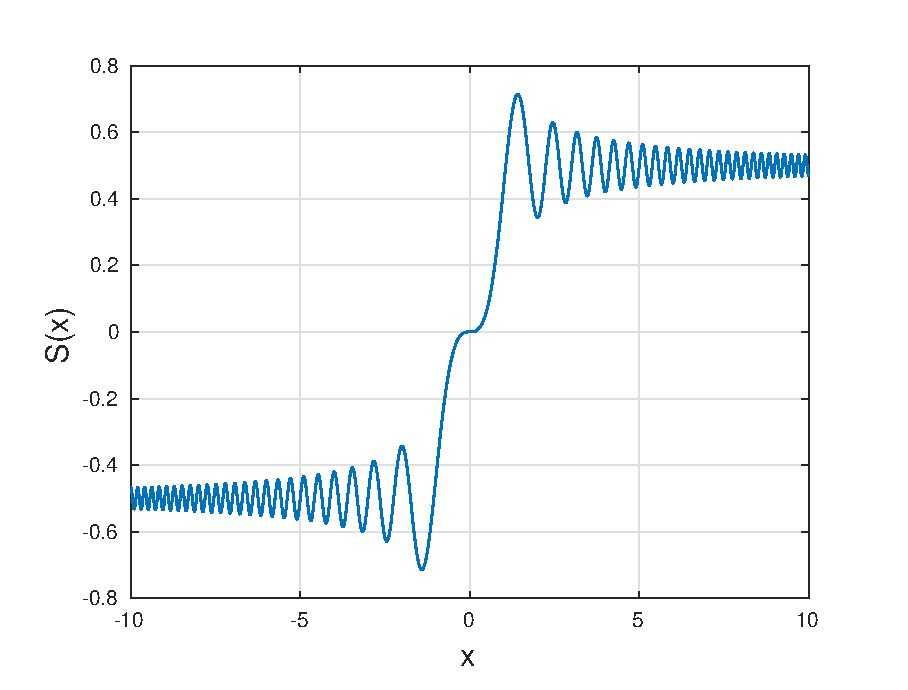
\includegraphics[scale=0.5]{fre2.eps}}
\subfigure[] {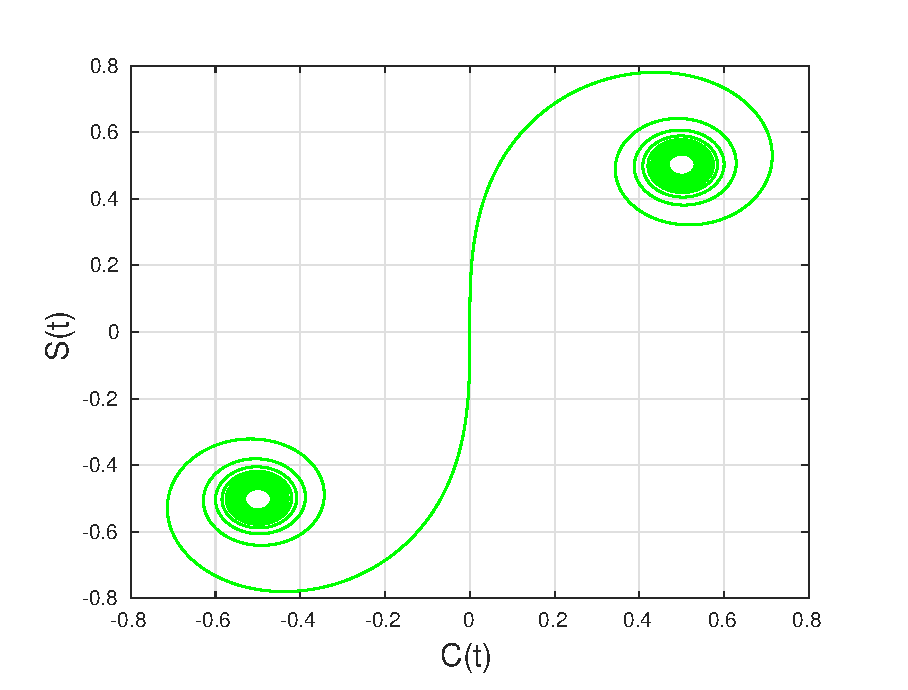
\includegraphics[scale=0.5]{curva.eps}}
\caption{integrales de fresnel (a.) y (b.); (c.) curva de Cornu }
\end{center}
\label{pos}
\end{figure}

\begin{figure*}[h!]
\begin{center}
\subfigure[] {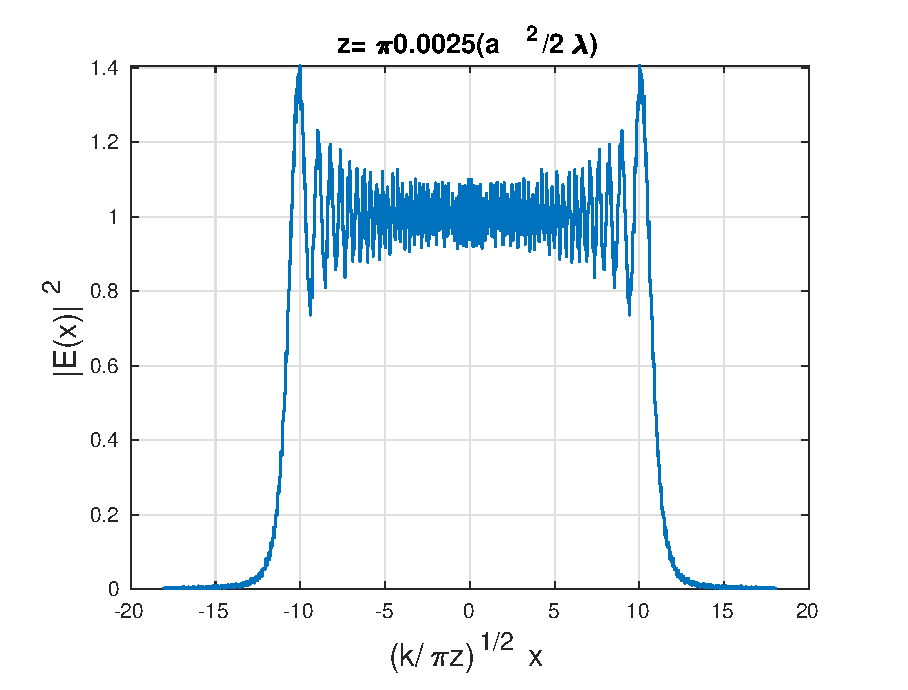
\includegraphics[scale=0.575]{p1.eps}}
\subfigure[] {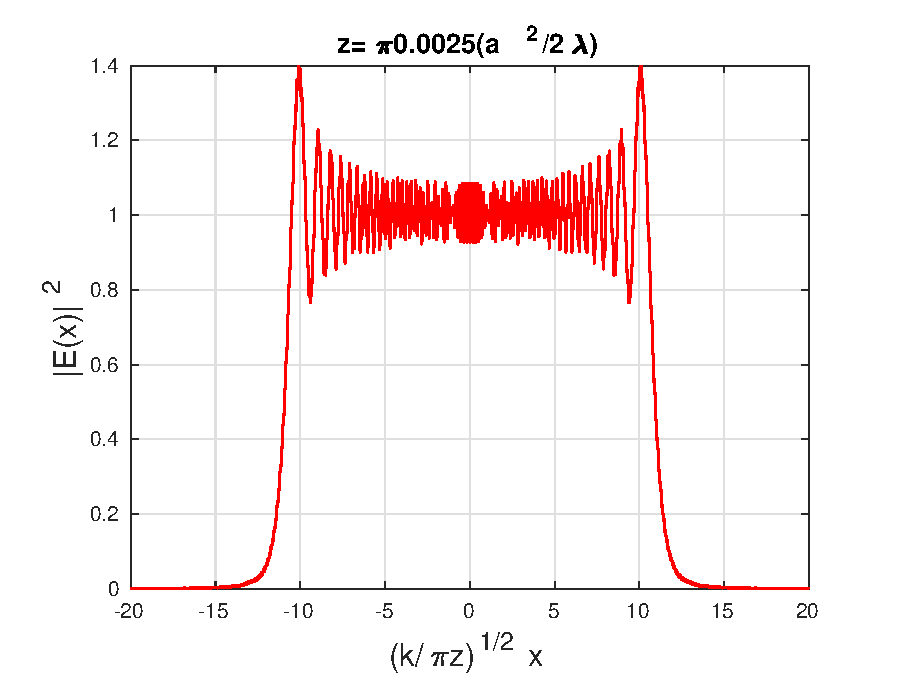
\includegraphics[scale=0.575]{p1t.eps}}\\
\subfigure[] {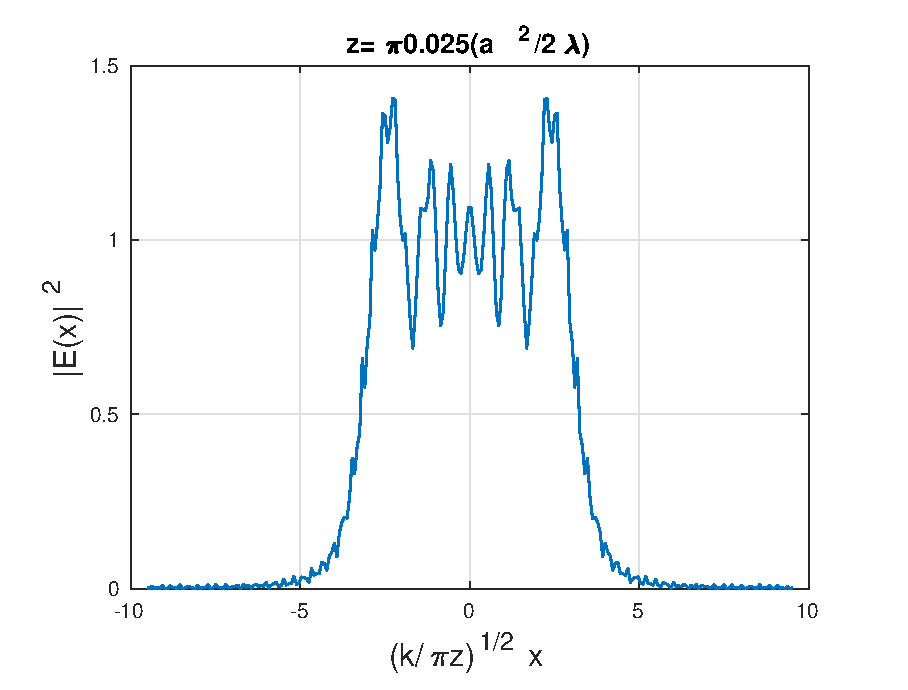
\includegraphics[scale=0.575]{p2.eps}}
\subfigure[] {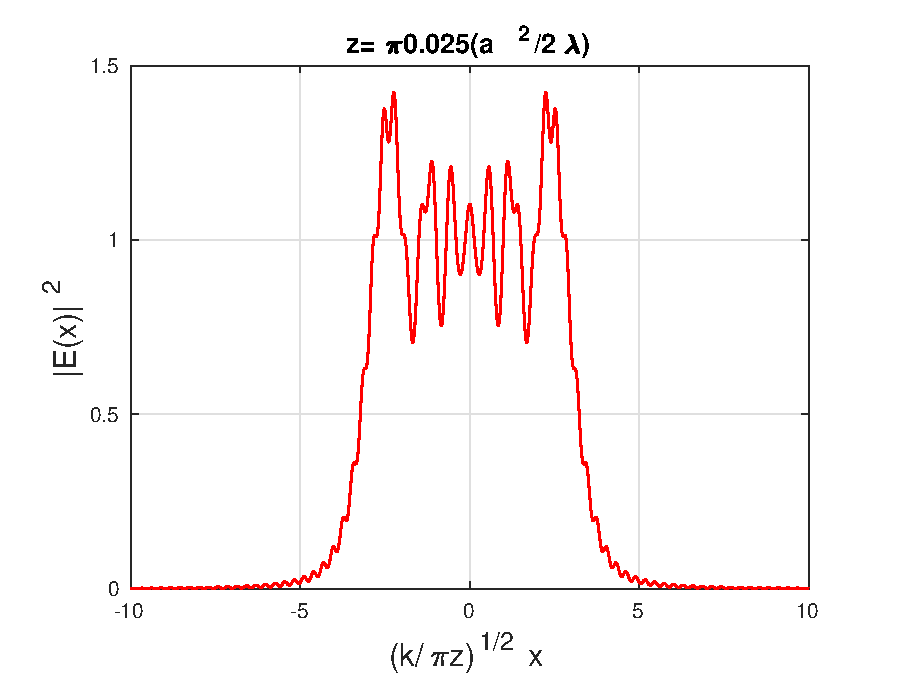
\includegraphics[scale=0.575]{p2t.eps}}\\
\subfigure[] {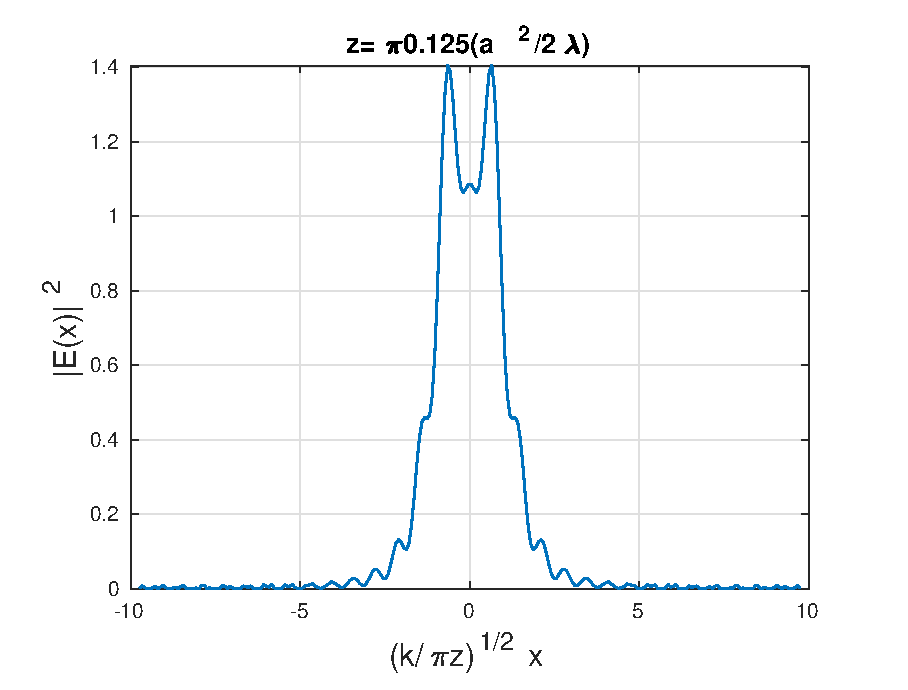
\includegraphics[scale=0.575]{p3.eps}}
\subfigure[] {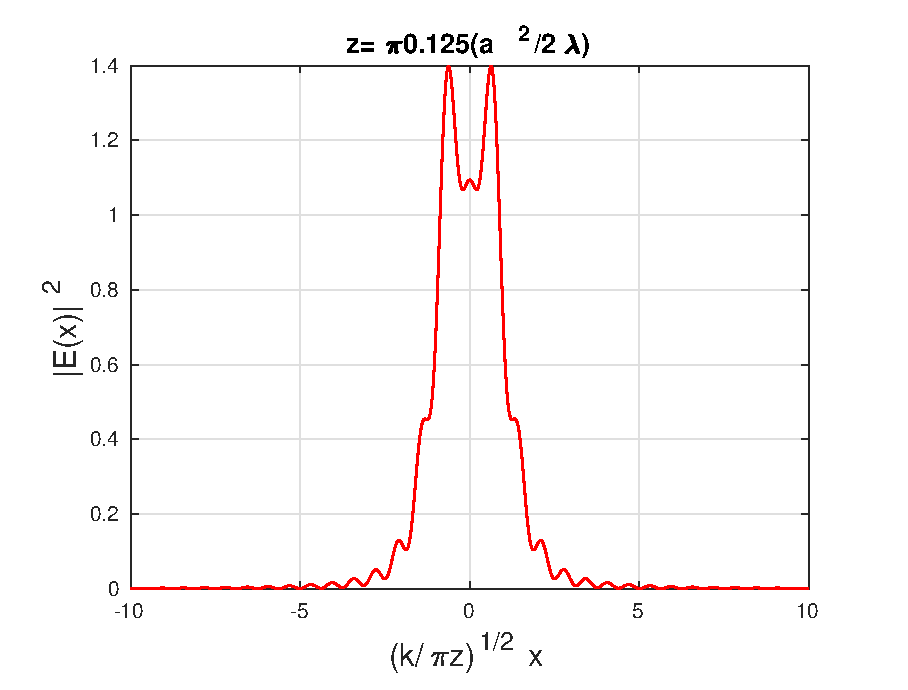
\includegraphics[scale=0.575]{p3t.eps}}\\
\caption{Patrones de difraccion de campo cercano y de transición para $a=0.075$ $[\mu m]$ y $\lambda=0.850$ $[\mu m]$. Del lado izquierdo se observan los patrones obtenidos y de lado derecho los patrones teoricos calculados.}
\end{center}
\label{pos}
\end{figure*}

\begin{figure*}[h!]
\begin{center}
\subfigure[] {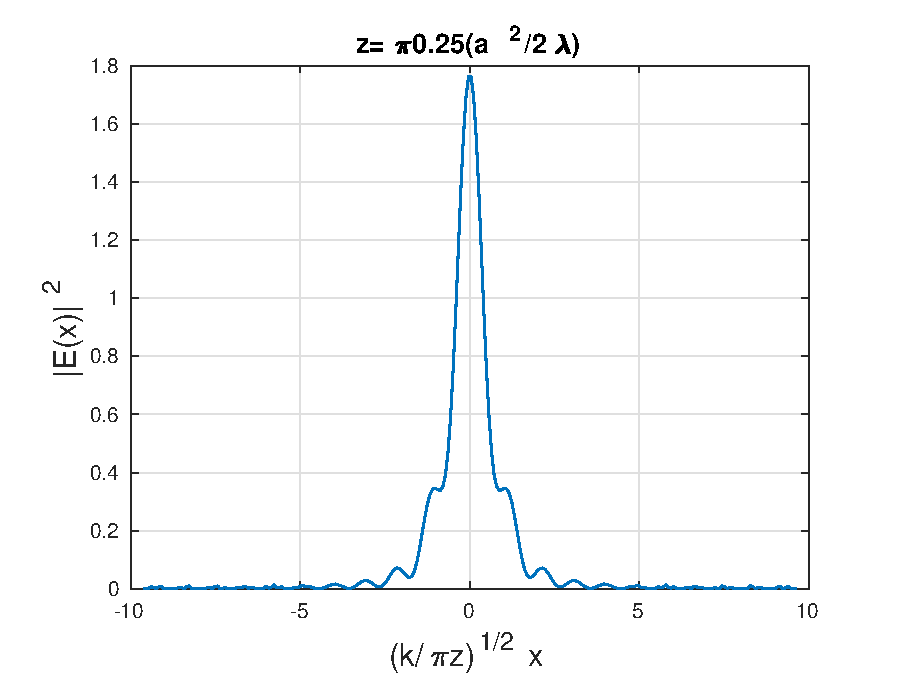
\includegraphics[scale=0.575]{p4.eps}}
\subfigure[] {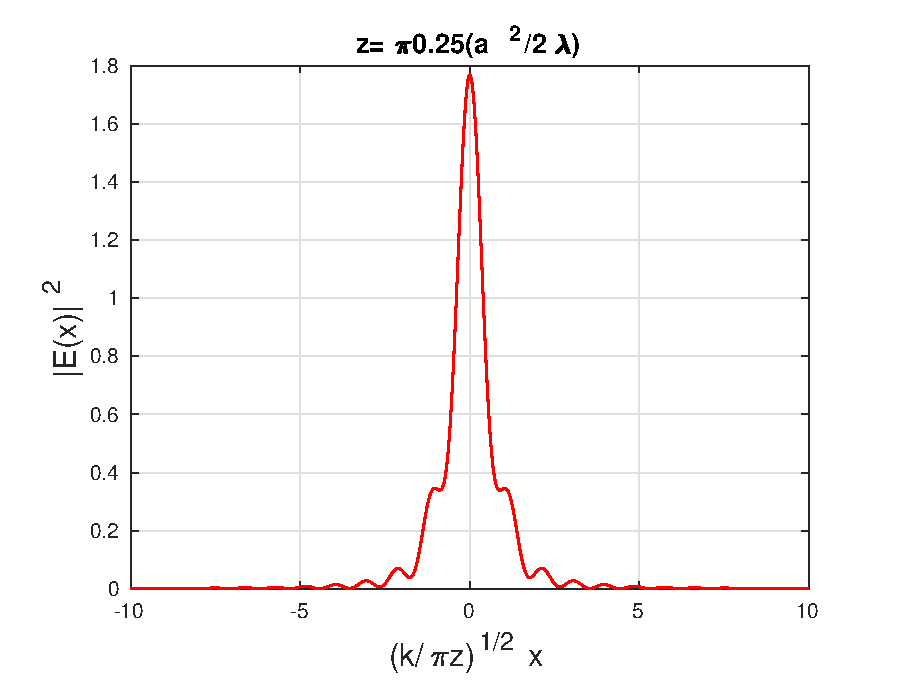
\includegraphics[scale=0.575]{p4t.eps}}\\
\subfigure[] {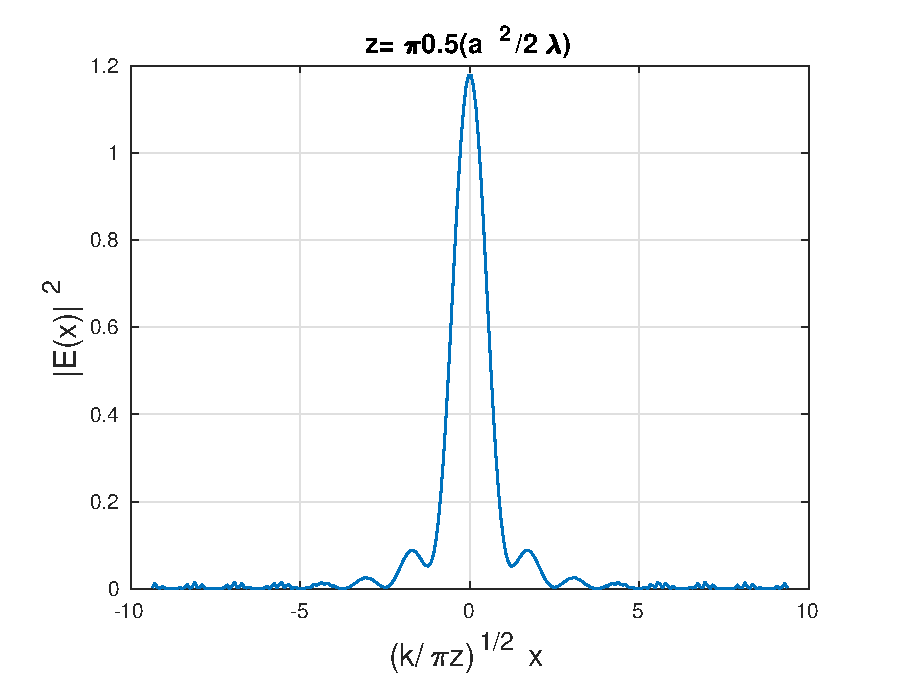
\includegraphics[scale=0.575]{p5.eps}}
\subfigure[] {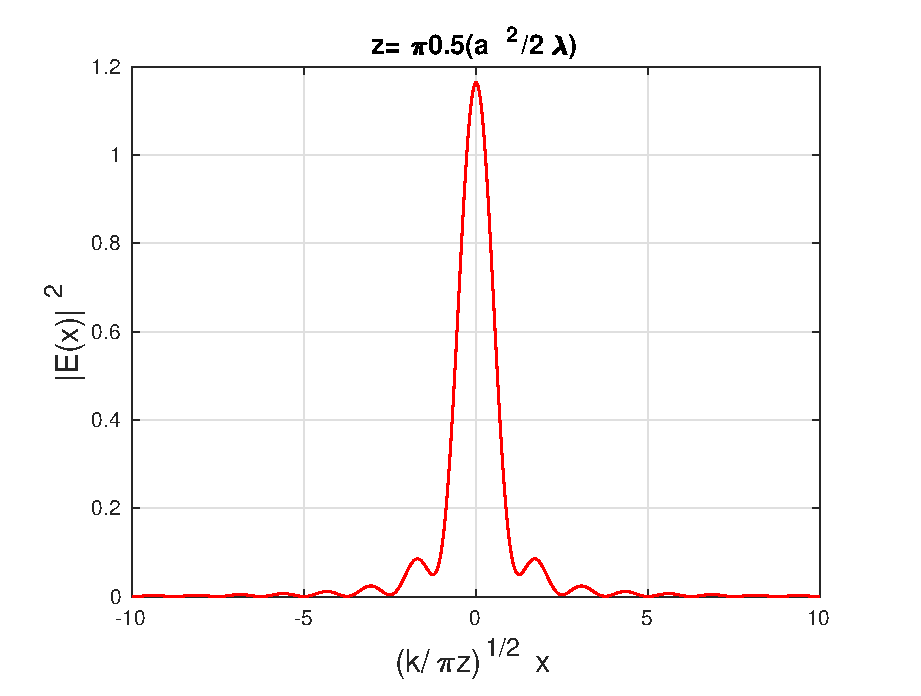
\includegraphics[scale=0.575]{p5t.eps}}\\
\subfigure[] {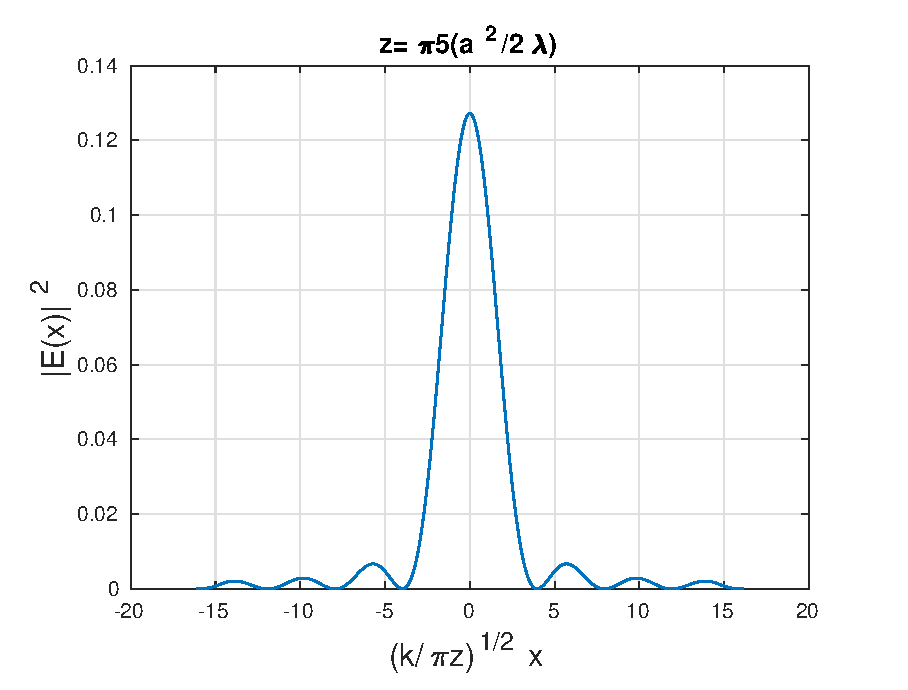
\includegraphics[scale=0.575]{p6.eps}}
\subfigure[] {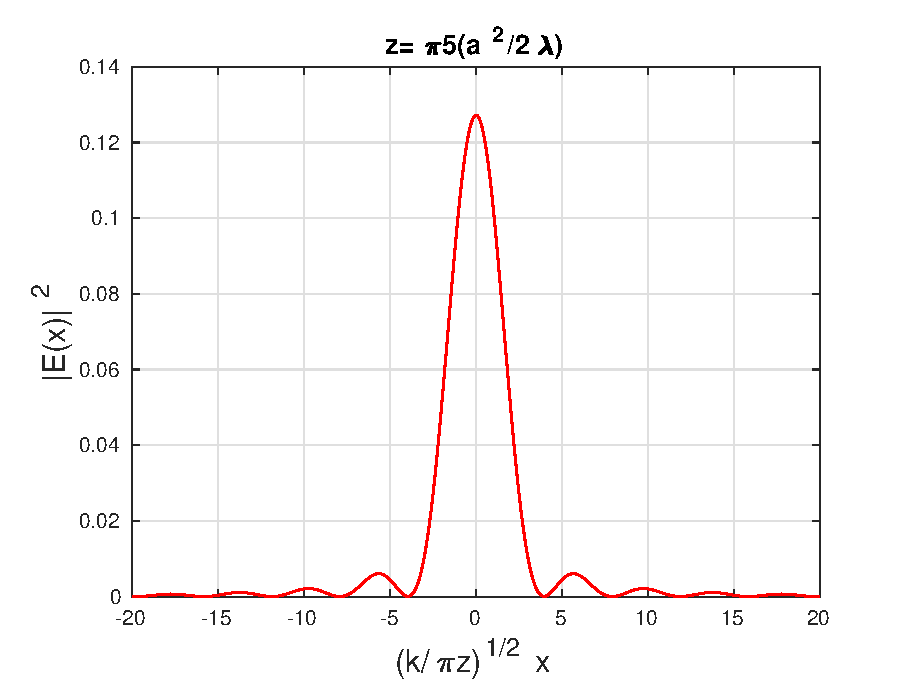
\includegraphics[scale=0.575]{p6t.eps}}\\
\caption{Patrones de difraccion campo lejano para $a=0.075$ $[\mu m]$ y $\lambda=0.850$ $[\mu m]$. Del lado izquierdo se observan los patrones obtenidos y de lado derecho los patrones teoricos calculados.}
\end{center}
\label{pos}
\end{figure*}
\par 
Ésta ultima grafica de la figura $(5)$ es la espiral de Cornu, también conocida como clotoide. Es la curva cuyas ecuaciones paramétricas vienen dadas por $S(x)$ y $C(x)$, tiene la propiedad de que su curvatura en cualquier punto es proporcional a la distancia a lo largo de la curva medida desde el origen. Esta propiedad hace que sea útil como curva de transición en el trazado de autopistas o ferrocarriles. En nuestro caso, al observar el argumento de las integrales en la ecuación (12), se aprecia como al disminuir $z$ éste argumento aumenta, provocando que los resultados de la integral se encuentren en la zonas de mayor oscilación (ver la figura 5 (a.) y (b.) ), obteniendo resultados muy diferentes para pequeñas variaciones del argumento a distancias muy cortas, lo cual con lleva a la forma de los patrones de difracción en campo cercano.\\
\par 
Finalmente, al comparar los datos obtenidos mediante la FFT (datos del lado izquierdo) con los patrones de difracción teóricos del problema (datos del lado derecho) en las figuras (6) y (7), se observa como éstos patrones de difracción son semejantes a los descritos por la teoría, presentando algunas diferencias mínimas o ``ruidos'' en campo cercano, debidos a la acumulación de información en pequeñas distancias. Es de apreciar, como el patrón de difracción cambia gradualmente de forma cuadrada (debida a la forma de la rendija), al patrón con máximos y mínimos de la teoría de Fraunhofer a medida que la distancia (de propagación) $z$ aumenta. El ruido observado en los patrones de campo cercano, en principio permite el poder justificar porqué muchas imágenes se observan ruidosas cuando son obtenidas a “cortas” distancias. El efecto difractivo se hace menos notorio para distancias muy grandes, aunque se pierde intensidad en la señal, lo cual en la practica dificultaría la reconstrucción de la imagen y/o señal inicial.

\section*{\normalsize{CONCLUSIÓN}}
Mediante las herramientas computacionales de MATLAB, se pudo estudiar, comparar y analizar los patrones de difracción que se producen cuando una onda plana atraviesa una rendija de tamaño finito $a$, tanto en campo cercano como lejano. Concluyendo que la transformada rápida de Fourier es una herramienta poderosa para la resolución de este tipo de problemas, que brinda la opción de observar y analizar los resultados predichos por la teoría de difracción de Fresnel y Fraunhofer. Observando que a menor distancia el patrón de difracción consigue definir de alguna manera el elemento difractante, en nuestro caso la rendija. Pero para distancias muy grandes el valor máximo de la intensidad de la radiación estará ubicado en la zona central del patrón. De manera similar, mediante la FFT se corroboro la dependencia de la cintura de un haz gaussiano a la distancia de propagación en la dirección $z$, con discrepancias menores al $1\%$ con respecto a lo predicho por la teoría de los haces gaussianos.
\section*{Referencias} 
\begin{itemize} 
\item[[ 1]] Daniel A. Steck. Classical and Modern Optics. Oregon Center for Optics and Department of Physics, University of Oregon, 2006. 
\item[[ 2]] Óscar Babilonia, Francisco Racedo, Sonia Valbuena. Análisis de la difracción por elementos cuadrados.Revista INGE CUC,Volumen 8, Número 1, Octubre de 2012, pp. 207-218.

\item[[ 3]]  William H. Press, Saúl A. Teukolsky, William T. Vetterling y Brian P. Flannery. Numerical Recipes: The Art of Scientific Computing. 

\item[[ 4]] O. Mata Méndez, Chávez Rivas. J. Sumaya Martínez. Teoría rigurosa de la dispersión de haces gaussianos por una rejilla con sustrato metálico. Superficies y Vacío 17(1), 27-31, marzo de 2004. 
\end{itemize}
\subsection*{Anexos}

\begin{lstlisting}
1. Codigo en MATLAB para 
la comprobacion de la 
teoria de haces gaussianos

% Asignacion de parametros
landa=0.532; k=2*pi/landa; 
wo=10; zo= (pi*wo.^2)/(landa);

N=2^11; x_f=5*wo; 
x=linspace(-x_f,x_f,N); 

% Condicion inicial
Eo=1;  
onda= Eo*exp(-(x.^2)/(wo.^2));

% Frecuencias
dx=(2*x_f)/N; 
n=-N/2:1:N/2; f=2*pi.*n/(N*dx); 
f=f(1:length(f)-1); 

% Transformada de Fourier 
transformada=fft(onda); 
transformada= fftshift(transformada) ; 

% Propagacion 
z=5e2;  
factor_propagador= 
exp(-(1i*(f.^2)*z)/(2*k));

onda_propagada1= 
transformada.*factor_propagador;

% Transformada inversa
transformada_inversa= 
ifft(ifftshift(onda_propagada1));
 
inversa_abs1=
abs(transformada_inversa);

%Energia
potencia_inicial= 
sum(abs(onda).^2)*dx ;  

potencia_final=
sum(inversa_abs1.^2)*dx ; 

$Fitting
[Cnts,ince]=
lsqcurvefit(@gau,[1,7],x
,inversa_abs1.^2); 

wzexp=Cnts(2);  
wz= wo*sqrt(1 + (z/zo).^2) ; 
Error_z= abs(wz-wzexp)/wz*100 ;

2. Codigo en MATLAB los 
patrones de difraccion 
utilizando el delta de Dirac, 
basado en el codigo de la seccion 1.

%Funcion que generaba el
delta de Dirac

function f=deltad(x,a,wo)
y=exp(-(x.^2)/(wo)); 
c=(a/2)>=x; d=x>=(-a/2); 
f= (c==d).*y; 
end

% utilizando el procedimiento anterior 
donde la nueva condicion inicial es    

onda= deltad(x,a,wo);

% Distancia a propagar

z=pi*5*((a.^2)/(2*landa))    

%Vizualizar el patron
plot(sqrt(k/(pi*z))*x,inversa_abs1.^2);

3. Determinacion teorica de los 
patrones de difraccion y las integrales de
fresnel.

% Condiciones 

xf=0; N=2e3; x= -xf:1e-2:xf; x1=x; 

%Paramettros
landa=0.850; a=0.075;
k=2*pi/landa; 
z=pi*5*(a.^2)/(2*landa); 
x= x./(sqrt(k/(pi*z))); 
Eo=1; 

I=[]; I2=[]; 
for n=1:length(x)

C=fresnelintegral(x1(n),N); 
S= fresnelintegral2(x1(n),N); 
    
datos1=[datos1,C];  
datos2=[datos2,S]; 
    
A= sqrt(k/(pi*z))*(x(n)+a/2); 
B= sqrt(k/(pi*z))*(x(n)-a/2); 
    
I1=(Eo.^2)/2*

( (fresnelintegral(A,N)-
fresnelintegral(B,N)).^2

 + (fresnelintegral2(A,N)-
 fresnelintegral2(B,N)).^2); 

I=[I,I1]; 
end

%visualizacion del patron de 
difraccion

plot(sqrt(k/(pi*z))*x,I,
'r','LineWidth',1.0); 

% Algoritmos que calcula las
integrales de fresnel

function f=fresnelintegral(x,N)
t=linspace(0,x,N); dt=x/N;  
int=cos(pi*t.^2/2); 
f=sum(int)*dt; 
end 

function f=fresnelintegral2(x,N)
t=linspace(0,x,N); dt=x/N;  
int=sin(pi*t.^2/2); 
f=sum(int)*dt; 
end 
\end{lstlisting}

\end{document}
